\documentclass{report}

\usepackage[backend=bibtex]{biblatex}
\usepackage[toc]{glossaries}
\usepackage{graphicx}
\usepackage{hyperref}
\usepackage{lmodern}
\usepackage{minted}
\usepackage{tabularx}
\usepackage{tcolorbox}

\newcommand{\code}[1]{\textsf{\ttfamily #1}}
\addbibresource{Rtutorial.bib}
\makenoidxglossaries

\newglossaryentry{dv}{name={discrete variable}, description={A variable that refers to categorical data (ex. color of eyes), as opposed to continuous data (ex. height in mm)}}
\newglossaryentry{cv}{name={continuous variable}, description={A variable that refers to continuous data, i.e. that can take on an infinite number of values (ex. height in mm), as opposed to categorical data (ex. color of eyes)}}
\newglossaryentry{ov}{name={ordinal variable}, description={A variable that refers to categorical data, but where the categories can be ordered (ex. small, medium, large)}}

\author{Myriam Luce}
\title{R: learn by the exercise}

\begin{document}
\maketitle
\tableofcontents

\chapter{Descriptive statistics}
	\section{Possibly interesting extra tidbits}
In the making of this tutorial, I used several tools that you might like to access as well. Being the tedium-averse programmer I am, I use a reference manager program, in my case Zotero. You can find the full bibliography for this project, including a few entries that did not make it into the references section here because I did not cite them, at \href{https://www.zotero.org/groups/2223910/r_tutorial}{the Zotero project page}.

I also want to point out \href{https://github.com/awesomedata/awesome-public-datasets}{awesome-public-datasets}, where I foraged for the examples in this tutorial. It has several interesting datasets in the public health domain.

	\section{Tables and figures}
	\subsection{Frequency table (1D) or contingency table (2D)}
If you feel the need to make a table with your data, use a spreadsheet software (Microsoft Excel, LibreOffice Calc, Google Sheets).  ;) R is superior in statistics and (arguably) in figures, but spreadsheets definitely have their uses when it comes to tables.
	\subsection{Pie chart}
A pie chart is a graph that can be used to visually represent proportions of a \emph{\gls{dv}}\footnote{Words in italics are defined in the glossary.}. Note that they have their critics, who recommend never using them, as our brain is bad at comparing the size of slices~\cite{wiki_pie}.

As an example data set, let's use ebola deaths by country~\cite{who}. An excerpt giving the source data is shown in figure~\ref{fig:ebola}. Enter the data in your favorite spreadsheet software and save it as a csv (thankfully for you English speakers, there is no need to fiddle with decimal symbol (is it a dot or a comma?) and whether the data is really comma-separated). You should get the following:
\begin{minted}{R}
Country,Deaths
Guinea,2543
Liberia,4809
Sierra Leone,3956
Mali,6
Nigeria,8
United States of America,1
\end{minted}
\begin{figure}[h]
	\centering
	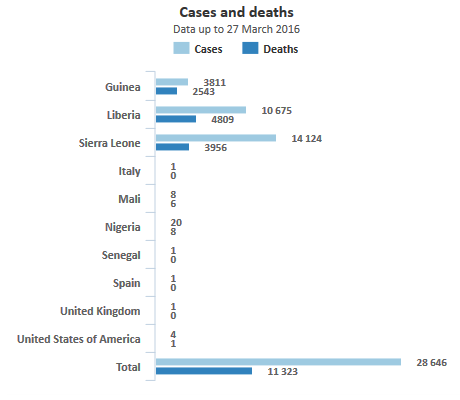
\includegraphics[width=0.8\textwidth]{ebola.png}
	\caption{Excerpt from \cite{who}.}
	\label{fig:ebola}
\end{figure}

R offers various data import options. The most useful I have found were \code{read.csv}\footnote{Words in monospace font refer to R commands. The cheat sheet at the end of the tutorial lists most of those used in this document.} to import csv data and \code{read.fwf} to import fixed-width data. To demonstrate, figure~\ref{fig:data} shows what csv (delimited) and fixed-width data look like side by side.
\begin{figure}[h]
	\centering
	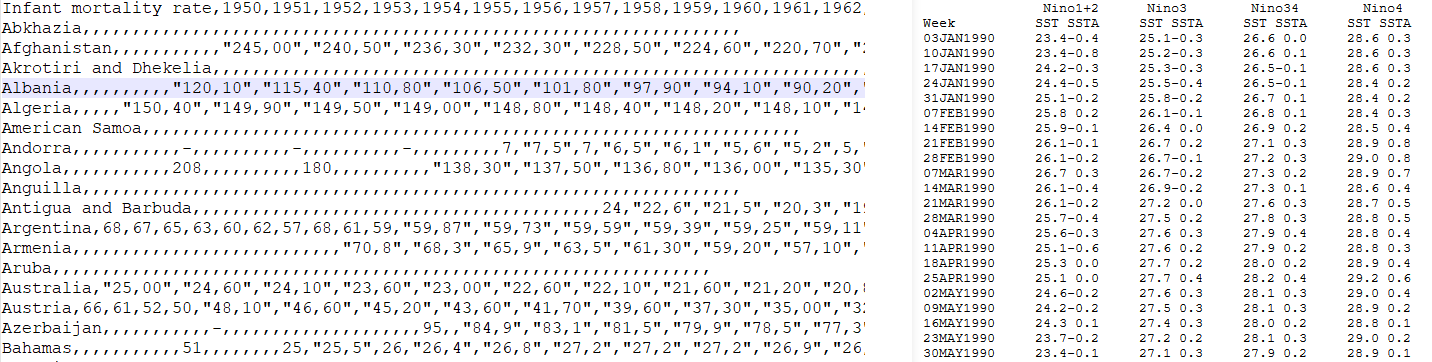
\includegraphics[width=1.0\textwidth]{data.png}
	\caption{Delimited data (left) and fixed-width data (right).}
	\label{fig:data}
\end{figure}

Go ahead and load your small csv into R with \code{read.csv('C:/......data.csv', header=TRUE)}. To avoid messing with default working folder in R settings, I recommend always using the full absolute file path (i.e. starting with C:). Note that you should use the \emph{forward slash "/"} as a path separator, even on Windows. The second parameter, \code{header=TRUE}, tells R that the first line in your file corresponds to the column headers, not actual data. You can then use the function \code{pie(counts, labels)} to produce a pie chart. However, as shown below, a naive approach might displease.
\begin{minted}{R}
> ebola = read.csv('D:/megha/Documents/r-tutorial/ebola.csv', header=TRUE)
> ebola
                   Country Deaths
1                   Guinea   2543
2                  Liberia   4809
3             Sierra Leone   3956
4                     Mali      6
5                  Nigeria      8
6 United States of America      1
> pie(ebola)
Error in pie(ebola) : 'x' values must be positive.
\end{minted}

You might be scratching your head and wondering which part of 2543 or 6 is not positive, and you'd be justified to do so. Here, one must dive into computer programming concerns to understand what is going on. The "not positive" message hints at a problem with the format of the input data. Let's demonstrate:
\begin{minted}[breaklines]{R}
> values = c(2543, 4809, 3956, 6, 8, 1
> labels = c('Guinea', 'Liberia', 'Sierra Leone', 'Mali', 'Nigeria', 'United States of America')
> pie(values, labels)	# works! produces figure 1.3
> typeof(values)
[1] "double"
> typeof(ebola)
[1] "list"
> class(values)
[1] "numeric"
> class(ebola)
[1] "data.frame"
> class(ebola$Country)
[1] "factor"
> class(ebola$Deaths)
[1] "integer"
> pie(ebola$Deaths, ebola$Country)	# works too now!

\end{minted}
\begin{figure}[h]
	\centering
	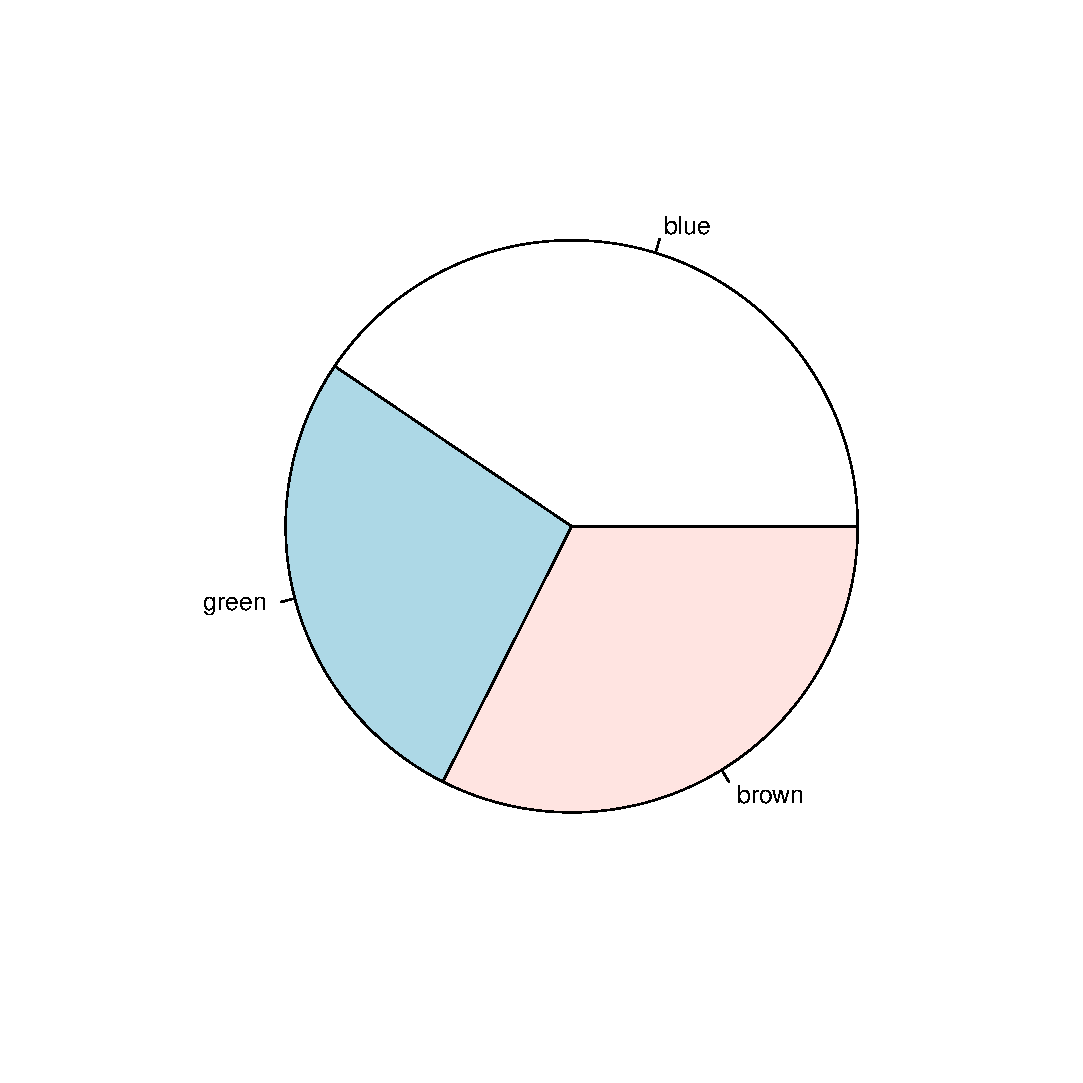
\includegraphics[width=0.8\textwidth]{pie.eps}
	\caption{Ebola deaths in 2015-2016 by country.}
\label{fig:pie}
\end{figure}

Technically, \code{read.csv} returns a \code{data.frame}, while \code{pie} only accepts numbers. Let's take a painful tangent into R types that will hopefully help you later on.

\begin{tcolorbox}[title=R types]
\begin{tabularx}{\textwidth}{>{\bfseries}l X}
Logical: & TRUE or FALSE\\[0.2cm]
Numeric: & real, by the math definition (ex. 12.3). Double is a numeric with better precision.\\[0.2cm]
Integer: & integer, by the math definition (ex. 12).\\[0.2cm]
Character: & text of any length\\[0.2cm]
Factor: & a type that represents a \gls{dv}\\[0.2cm]
Ordered: & a type that represents an \gls{ov}\\[0.2cm]
List: & a 1D collection of "things" (may be strings, numbers, or a mix of them)\\[0.2cm]
Vector: & a 1D collection of things of \emph{one type}\\[0.2cm]
Matrix: & a 2D collection of things of \emph{one type}\\[0.2cm]
Array: & a nD collection of things of \emph{one type}\\[0.2cm]
Data Frame: & a (mostly) 2D collection of things, where each column can be of a different type
\end{tabularx}
For future reference, Quick R gives an excellent introduction on the subject~\cite{quickr}. You can convert a variable to anything reasonable (R will turn "2" into an integer, but not "abc") using the host of \code{as.xyz} functions.
\end{tcolorbox}
\begin{tcolorbox}[title=Accessing collection elements]
Let's say you have a data frame, for example your ebola deaths by country data:
\begin{minted}[breaklines]{R}
> ebola
                   Country Deaths
1                   Guinea   2543
2                  Liberia   4809
3             Sierra Leone   3956
4                     Mali      6
5                  Nigeria      8
6 United States of America      1
\end{minted}
Notice how the line with "Country" and "Deaths" is not numbered in the output? It means R is aware it's a header and not data. Data frame columns can be accessed by their name using the \code{\$} operator, like so:
\begin{minted}[breaklines]{R}
> ebola$Country
[1] Guinea                   Liberia                  Sierra Leone            
[4] Mali                     Nigeria                  United States of America
6 Levels: Guinea Liberia Mali Nigeria ... United States of America
\end{minted}
If you want to access lines, you can use the \code{[row, column]} operator, like so:
\begin{minted}[breaklines]{R}
> ebola[1,]
  Country Deaths
1  Guinea   2543
> ebola[1,2]
[1] 2543
\end{minted}
While the \code{\$} operator is exclusive to data frames, the \code{[]} is used for all collections. Vectors, lists, matrices and arrays can be accessed with the \code{[index]} operator for 1D structure, \code{[row, column]} operator for 2D structures, and \code{[i, j, k...]} for nD structures.

In the case you want to access several items at once, you can use a colon inside the brackets, i.e. \code{[begin:end]} like so:
\begin{minted}[breaklines]{R}
> ebola[1:3,]
       Country Deaths
1       Guinea   2543
2      Liberia   4809
3 Sierra Leone   3956
\end{minted}
\end{tcolorbox}

Now that we have our basic pie chart, you might be thinking, "That squiggle on the right with the tiny pie slices is quite unseemly". In addition, you might want to tweak other aspects of the graph, like adding a title or choosing colors. We will discuss common graph properties in a following section, to keep it all in the same place. Let's just deal with the pie-chart specific problem of small slices here (I reiterate, you should run away, run away into the arms of a bar chart.), and add a percent annotation, as that is a common occurence. R does not offer an option to deal with small slices out of the box (probably because it tells you in its own manual to use bar charts instead), so let's just manually tweak the labels:
\begin{minted}[breaklines]{R}
> labels = as.character(ebola$Country)
> labels[4]='Others'
> labels[5:6]=''
> labels
[1] "Guinea"       "Liberia"      "Sierra Leone" "Others"       ""            
[6] ""
> percents = ebola\$Deaths/sum(ebola\$Deaths)*100
> percents
[1] 22.458712355 42.471076570 34.937737349  0.052989490  0.070652654
[6]  0.008831582
> percents[4] = sum(percents[4:6])
> percents
[1] 22.458712355 42.471076570 34.937737349  0.132473726  0.070652654
[6]  0.008831582
> percents = round(percents, 2)
> percents
[1] 22.46 42.47 34.94  0.13  0.07  0.01
> labels[1:4] = paste(labels[1:4], percents[1:4], '\%')
> labels
[1] "Guinea 22.46 \%"       "Liberia 42.47 \%"      "Sierra Leone 34.94 \%"
[4] "Others 0.13 \%"
> pie(ebola\$Deaths, labels)
\end{minted}
Hacky, but it works, and no more time should be dedicated to pie charts, so let's move on.

	\subsection{Bar chart}
A bar chart, sometimes called a line graph, is used to represent a \gls{dv}, and the bars \emph{do not touch}. As an example, data on infant mortality by country can be found at \href{https://docs.google.com/spreadsheets/d/1OHMMuHbSFKDolNHXsmgHYlkjSKfAZyyY1P-ddMu_Fz0/pub}{Gapminder}~\cite{gapminder}. If you simply \code{read.csv} the file you just downloaded and converted to csv using your favorite Spreadsheet software, and then examine the structure of your data inside R, you might notice the somewhat strange following occurence:
\begin{minted}[breaklines]{R}
> infant = read.csv('D:/megha/Documents/r-tutorial/infant.csv', header=TRUE)
> class(infant)
[1] "data.frame"
> str(infant)
'data.frame':   260 obs. of  217 variables:
 $ Infant.mortality.rate: Factor w/ 260 levels "Abkhazia","Afghanistan",..: 1 2 3 5 6 7 8 9 10 11 ...
 $ X1800                : int  NA NA NA NA NA NA NA NA NA NA ...
 $ X1801                : int  NA NA NA NA NA NA NA NA NA NA ...
# ...
 $ X1861                : int  NA NA NA NA NA NA NA NA NA NA ...
 $ X1862                : Factor w/ 11 levels "",".","110","131",..: 1 1 1 1 1 1 1 1 1 1 ...
 $ X1863                : Factor w/ 13 levels "",".","106","113",..: 1 1 1 1 1 1 1 1 1 1 ...
# ... 
\end{minted}

Wait, what? The country is of type factor, we all agree on that, but infant mortality rate for 1862 is a factor? Using good ol' Notepad or a better text editor, open your csv and scroll around, you should spot the problem illustrated in figure~\ref{fig:welcome}.
\begin{figure}[h]
	\centering
	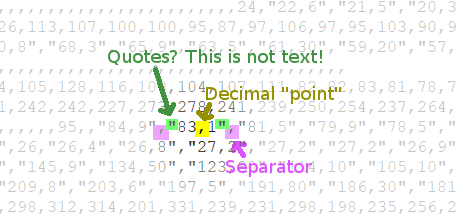
\includegraphics[width=1.0\textwidth]{welcometotherealworld.png}
	\caption{Welcome to the real world. CSV sucks internationally.}
\label{fig:welcome}
\end{figure}

In other languages, like French for instance, the decimal "point" is a comma, and therefore the "comma-separated" part of comma-separated value leads to some issues. Other gems in this data include "-" for I assume missing data, and some lonely dots, assuming again, for missing data. Gods forbid the authors hit a snag while importing data and their software didn't warn them something foul was afoot and they just pasted it in the global csv without noticing. (This is why science should be in databases. Real databases. They don't let you put a dash in a number field, they just don't.)

Thankfully, \code{read.csv} comes with some handy options. You can see them all in the manual by typing \code{?read.csv} in a R console. So, we need to tell R that our \code{dec} point is a comma, and dash and dot stand for missing data, i.e. \code{na.strings}. Technically, R also thinks that things surrounded by quotes are text, but is smart enough to automatically check if the "text" looks like a number and, if it does, it converts it automatically to a number. You therefore get the appropriate following:
\begin{minted}[breaklines]{R}
> infant = read.csv('D:/megha/Documents/r-tutorial/infant.csv', header=TRUE, dec=",", na.strings=c('-', '.'))
> str(infant)
'data.frame':   260 obs. of  217 variables:
 $ Infant.mortality.rate: Factor w/ 260 levels "Abkhazia","Afghanistan",..: 1 2 3 5 6 7 8 9 10 11 ...
 $ X1800                : int  NA NA NA NA NA NA NA NA NA NA ...
 $ X1801                : int  NA NA NA NA NA NA NA NA NA NA ...
 # ...
 \end{minted}

A barplot is relatively straightforward to produce with R, but we will see all "common" (imho) plot options here, so tie your winter hat down with wire, you'll be sitting here a while.  Let's start by simply plotting infant mortality rate by country. To keep the plot readable, let's choose a subset of G8 countries: Canada, France, Germany, Italy, Japan, Russia, United Kingdom and United States of America. Let's also start by studying the mortality rate in 2000. First, we will select each of the countries by its row number, then we will stitch the G8 back together with a function called \code{rbind}, which binds data frames together by row, as long as all data frames have the same columns.
\begin{minted}[breaklines]{R}
> canada = infant[38,]
> france = infant[77,]
> germany = infant[83,]
> italy = infant[109,]
> japan = infant[111,]
> russia = infant[186,]
> uk = infant[240,]
> usa = infant[241,]
> g8 = rbind(canada, france, germany, italy, japan, russia, uk, usa)
 \end{minted}

Producing a barplot now is easy:
\begin{minted}[breaklines]{R}
> barplot(g8$X2000, names.arg=g8$Infant.mortality.rate)
 \end{minted}
\begin{figure}[h]
	\centering
	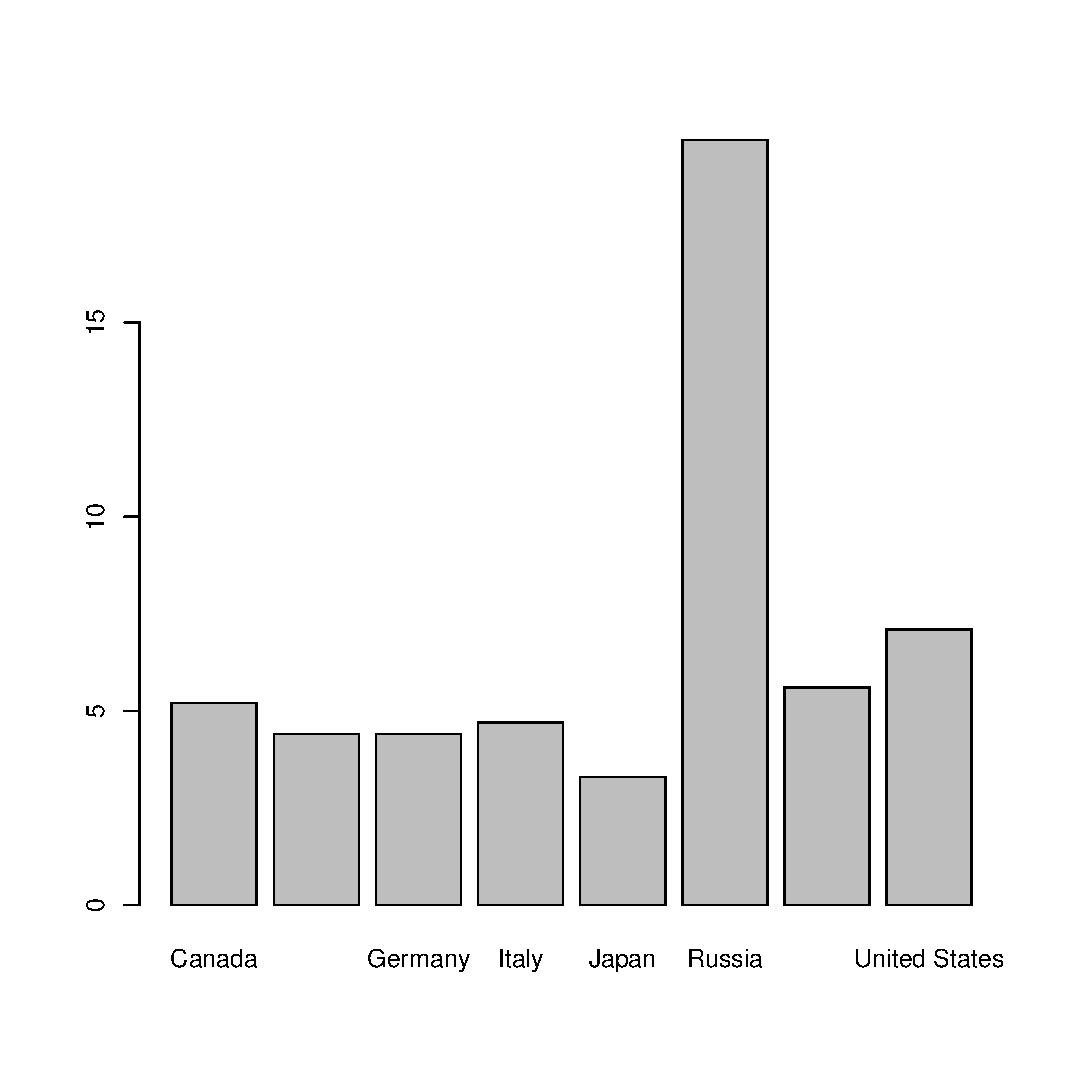
\includegraphics[width=1.0\textwidth]{barsimple.eps}
	\caption{Simplest bar plot: infant mortality rate per country.}
\label{fig:simplebar}
\end{figure}

Several things are wrong with this graph. Glaringly, a bar should not extend beyond its axis. Axes are set as plot options with \code{xlim} and \code{ylim}. Also, should you want a box around the graph, \code{bty} takes care of that. Usually. Bar plots are special and you need to all an extra function after your plot appears. See all graph options with \code{?par}, which we will use a lot more as we customize our graphs.
\begin{minted}[breaklines]{R}
barplot(g8$X2000, names.arg=g8$Infant.mortality.rate, ylim=c(0,20), bty='o')	# why oh why won't bty work like everywhere else!
box()
 \end{minted}
\begin{figure}[h]
	\centering
	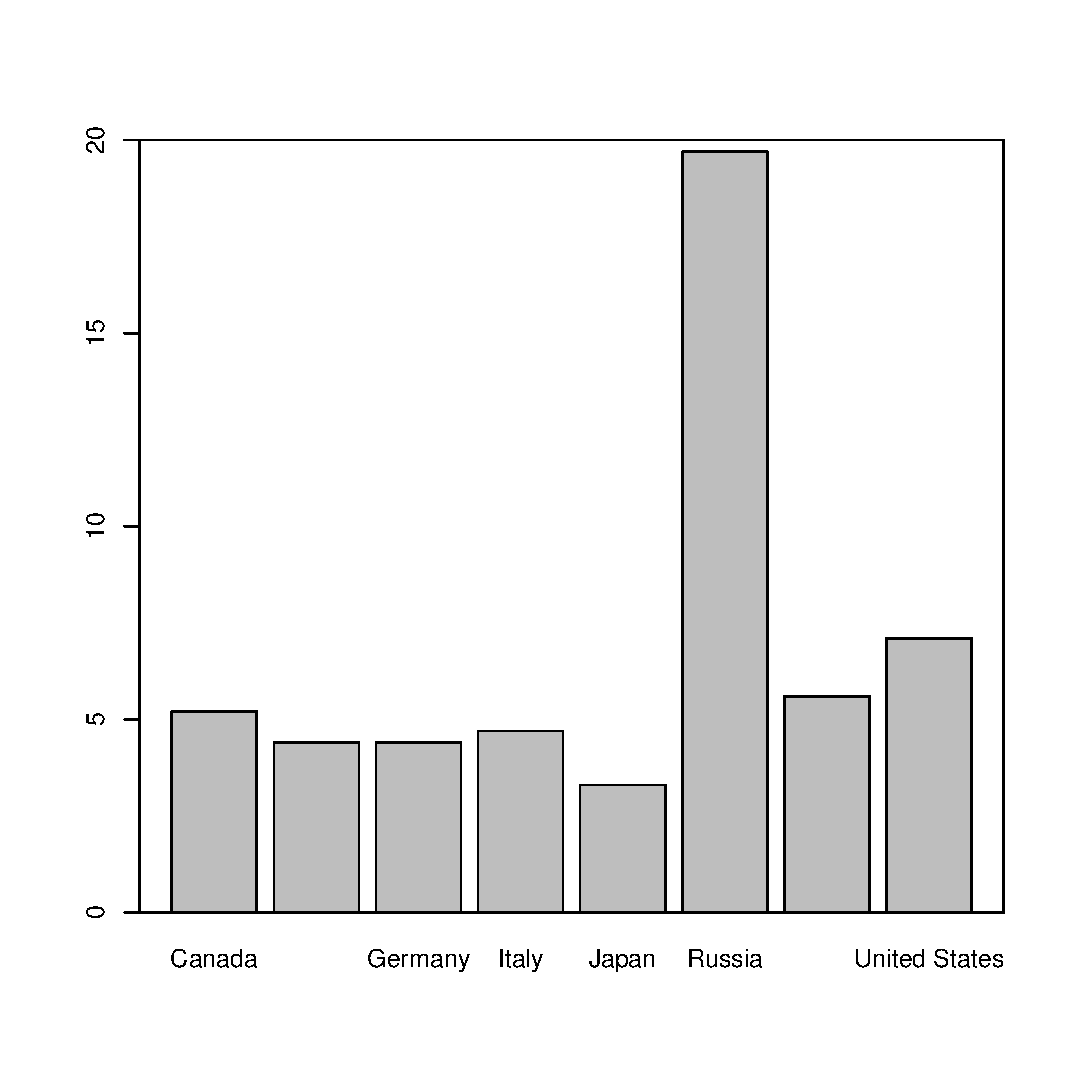
\includegraphics[width=1.0\textwidth]{baraxis.eps}
	\caption{Simple bar plot: infant mortality rate per country, axis set.}
\label{fig:baraxis}
\end{figure}

You probably also want all country names to show up. Easiest way to do that is to tilt the axis label text. Enter \code{par}, used \emph{before} your graph function to set general settings. For this next iteration, let's do a few things at once. First, let's make all labels perpendicular to their axis with \code{par} and \code{las}. Let's also demonstrate color manipulation by making each country's bar the dominant color on their flag (this might lead to arbitrary choices) with \code{col}.
\begin{minted}[breaklines]{R}
> colors = c('red', 'blue', 'black', 'green', 'white', 'snow', 'purple', 'purple4')
> par(las=2)		# axis labels: perpendicular
> barplot(g8$X2000, names.arg=g8$Infant.mortality.rate, ylim=c(0,20), col=colors)
> box()
\end{minted}

\begin{tcolorbox}[title=Colors in R, parbox=false]
Colors in R can be specified by their names, if they are among R's list of approved colors, which you can see by calling \code{colors()}.

A more visually helpful version can be found at \href{http://research.stowers.org/mcm/efg/R/Color/Chart/}{Color Chart}~\cite{rcolors} which, incidentally, has other fascinating references about the use of color in science (good vs. bad color ramps, color blindness considerations).

Additionally, colors can be specified in other formats like \code{\#RRGGBB} where 00 $\leq$ color $\leq$ FF. These values can be found with graphics software or off a color generator on the internet.

Finally, if color space is a factor, additional functions exist: \code{rgb}, \code{hsv}, \code{hcl}, \code{gray} and \code{rainbow}.
\end{tcolorbox}

\begin{figure}[h]
	\centering
	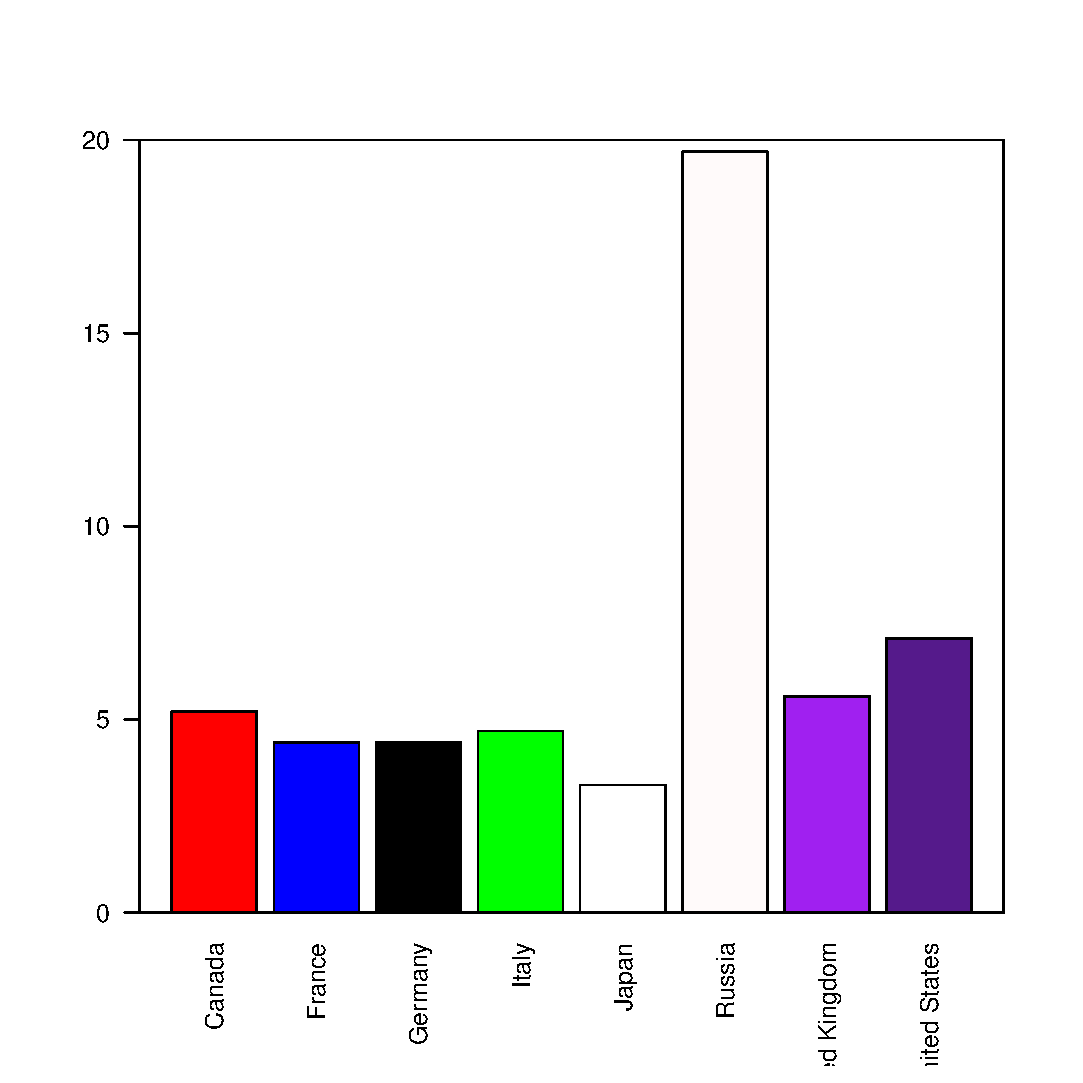
\includegraphics[width=1.0\textwidth]{barpsych.eps}
	\caption{Psychedelic bar plot: infant mortality rate per country, axis set, labels perpendicular, colors.}
\label{fig:barpsych}
\end{figure}

With the country names printed at the vertical, they are running out of space at the bottom of the graph. More margin is needed there. Figures have two types of margins in R: outer and inner. The inner margin is used to draw the figure title and the axis ticks and labels and can be set in inches with \code{mai=c(bottom, left, top, right)} or in lines with \code{mar=c(bottom, left, top, right)}. The outer margin is outside the figure; it makes more sense when several plots are displayed together, as we will do a few exercises down the line. The outer margin as well can be set in inches with \code{omi=c(bottom, left, top, right)} or in lines with \code{oma=c(bottom, left, top, right)}. As for the appropriate margin necessary to display the full country name, that's a matter of trial and error. Starting with the current parameters' value of inner margin, I found that a value of 8 worked well.
\begin{minted}[breaklines]{R}
par()$mar
[1] 5.1 4.1 4.1 2.1
> par(mar=c(8, 4.1, 4.1, 2.1))
> barplot(g8$X2000, names.arg=g8$Infant.mortality.rate, ylim=c(0,20), col=colors)
> box()
\end{minted}


	\subsection{Histogram}
	\subsection{Line graph}
	\subsection{Scatter graph}
	\subsection{Box and whiskers graph}
	\section{Numbers}
	\subsection{Center}
	\subsubsection{Mean}
	\subsubsection{Median}
	\subsubsection{Mode}
	\subsection{Dispersion}
	\subsubsection{Range}
	\subsubsection{Variance}
	\subsubsection{Standard deviation}
	\subsubsection{Coefficient of variation}
	\subsubsection{Quartiles and percentiles}
	\subsection{Shape}
	\subsubsection{Skewness}
	\subsubsection{Kurtosis}
	\subsubsection{L-moments}

\chapter{Probabilities}
	\section{Factorial}
	\section{Combinations}
	\section{Permutations}
	\section{Probability Mass/Density Function}

\chapter{Statistics}
	\section{Binomial distribution}
	\section{Multinomial distribution}
	\section{Poisson distribution}
	\section{Inverse binomial distribution}
	\section{Hypergeometric distribution}
	\section{Normal distribution}
	\section{Exponential distribution}
	\section{Gamma distribution}
	\section{c2 distribution}
	\section{Fisher-Snedecor distribution}
	\section{Student’s law}

\chapter{Inferential statistics}
	\section{Student’s test}
	\section{Student’s paired test}
	\section{Bartlett’s test}
	\section{Single-factor ANOVA}
	\section{c2 test}
	\section{Wilcoxon-Mann-Whitney test}
	\section{Kolmogorov-Smirnov test}
	\section{Kruskal-Wallis test}
	\section{Pearson’s test}
	\section{Spearman’s test}
	\section{Kendall’s test}
	\section{Simple linear regression}
	\section{Multiple linear regression}

\chapter{Cheat sheet}

	\section{Plumbing}
\begin{tabbing}
?~~~~~~~~~~~~~ \= ?exact\_function\_name \\
?? \> ??keyword \\
typeof \> typeof(R\_variable) \\
class \> class(R\_variable) \\
str \> str(R\_variable) \\
colnames \> colnames(R\_variable) \\
as.integer \> as.integer(R\_variable)
\end{tabbing}

	\section{Data import and export}
\begin{tabbing}
read.csv~~~~ \= read.csv('delimited\_data.csv', header=TRUE, sep=",", dec=".") \\
read.fwf \> read.fwf('fixed\_width\_data.txt', widths=c(10, 5, 4), header=TRUE, skip=2) \\
write.csv \> write.csv(R\_variable, file='desired\_file\_name.csv', append=FALSE)
\end{tabbing}

\printbibliography

\printnoidxglossaries

\end{document}